% Options for packages loaded elsewhere
\PassOptionsToPackage{unicode}{hyperref}
\PassOptionsToPackage{hyphens}{url}
%
\documentclass[
]{article}
\usepackage{amsmath,amssymb}
\usepackage{lmodern}
\usepackage{iftex}
\ifPDFTeX
  \usepackage[T1]{fontenc}
  \usepackage[utf8]{inputenc}
  \usepackage{textcomp} % provide euro and other symbols
\else % if luatex or xetex
  \usepackage{unicode-math}
  \defaultfontfeatures{Scale=MatchLowercase}
  \defaultfontfeatures[\rmfamily]{Ligatures=TeX,Scale=1}
\fi
% Use upquote if available, for straight quotes in verbatim environments
\IfFileExists{upquote.sty}{\usepackage{upquote}}{}
\IfFileExists{microtype.sty}{% use microtype if available
  \usepackage[]{microtype}
  \UseMicrotypeSet[protrusion]{basicmath} % disable protrusion for tt fonts
}{}
\makeatletter
\@ifundefined{KOMAClassName}{% if non-KOMA class
  \IfFileExists{parskip.sty}{%
    \usepackage{parskip}
  }{% else
    \setlength{\parindent}{0pt}
    \setlength{\parskip}{6pt plus 2pt minus 1pt}}
}{% if KOMA class
  \KOMAoptions{parskip=half}}
\makeatother
\usepackage{xcolor}
\IfFileExists{xurl.sty}{\usepackage{xurl}}{} % add URL line breaks if available
\IfFileExists{bookmark.sty}{\usepackage{bookmark}}{\usepackage{hyperref}}
\hypersetup{
  pdftitle={Drone Strikes in the Middle East},
  pdfauthor={Ethan Allavarpu},
  hidelinks,
  pdfcreator={LaTeX via pandoc}}
\urlstyle{same} % disable monospaced font for URLs
\usepackage[margin=1in]{geometry}
\usepackage{graphicx}
\makeatletter
\def\maxwidth{\ifdim\Gin@nat@width>\linewidth\linewidth\else\Gin@nat@width\fi}
\def\maxheight{\ifdim\Gin@nat@height>\textheight\textheight\else\Gin@nat@height\fi}
\makeatother
% Scale images if necessary, so that they will not overflow the page
% margins by default, and it is still possible to overwrite the defaults
% using explicit options in \includegraphics[width, height, ...]{}
\setkeys{Gin}{width=\maxwidth,height=\maxheight,keepaspectratio}
% Set default figure placement to htbp
\makeatletter
\def\fps@figure{htbp}
\makeatother
\setlength{\emergencystretch}{3em} % prevent overfull lines
\providecommand{\tightlist}{%
  \setlength{\itemsep}{0pt}\setlength{\parskip}{0pt}}
\setcounter{secnumdepth}{-\maxdimen} % remove section numbering
\usepackage{booktabs}
\usepackage{longtable}
\usepackage{array}
\usepackage{multirow}
\usepackage{wrapfig}
\usepackage{float}
\usepackage{caption}
\usepackage{colortbl}
\usepackage{pdflscape}
\usepackage{tabu}
\usepackage{threeparttable}
\usepackage{threeparttablex}
\usepackage[normalem]{ulem}
\usepackage{makecell}
\usepackage{xcolor}
\usepackage{booktabs}
\usepackage{longtable}
\usepackage{array}
\usepackage{multirow}
\usepackage{wrapfig}
\usepackage{float}
\usepackage{colortbl}
\usepackage{pdflscape}
\usepackage{tabu}
\usepackage{threeparttable}
\usepackage{threeparttablex}
\usepackage[normalem]{ulem}
\usepackage{makecell}
\usepackage{xcolor}
\ifLuaTeX
  \usepackage{selnolig}  % disable illegal ligatures
\fi

\title{Drone Strikes in the Middle East}
\usepackage{etoolbox}
\makeatletter
\providecommand{\subtitle}[1]{% add subtitle to \maketitle
  \apptocmd{\@title}{\par {\large #1 \par}}{}{}
}
\makeatother
\subtitle{Pakistan, Somalia, Yemen}
\author{Ethan Allavarpu}
\date{3 June 2022}

\begin{document}
\maketitle

{
\setcounter{tocdepth}{1}
\tableofcontents
}
\vfill

\hypertarget{abstract}{%
\section{Abstract}\label{abstract}}

In this report, we look at drone strike data from 2004 onward (Pakistan)
and 2007 onward (Somalia and Yemen). We consider the distribution of
civilian casualties by country and president in addition to frequency of
strikes by president. Our analyses indicate that Pakistan had a higher
percentage of civilian casualties, while Somalia had a civilian casualty
rate (as a percent of the total persons killed) distinctly less than
expected. Regarding presidents, we find evidence that the lethality of
drone strikes differs by president (with Bush having the largest average
fatality per strike), but do not find evidence of a significant
difference in drone frequency by term length.

\pagebreak

\hypertarget{background}{%
\section{Background}\label{background}}

\hypertarget{context}{%
\subsection{Context}\label{context}}

\hypertarget{data-introduction}{%
\subsection{Data Introduction}\label{data-introduction}}

The data contains information on drone strikes in the Middle East,
courtesy of The Guardian. We have drone strike data since 2004 for
Pakistan and from 2007 for Somalia and Yemen. Within these datasets,
each observation corresponds to a single drone strike. We have
information on the date and area of the strike along with the number of
people, civilians, and children killed and the number of people injured.

From the area and country for each strike, we used a Google Maps API key
(within the \texttt{ggmap()} package) to geocode the areas into latitude
and longitude. The latitude and longitude are for a general area--not a
specific strike location--and some observations did not have geocoded
locations.

\hypertarget{exploratory-data-analysis}{%
\section{Exploratory Data Analysis}\label{exploratory-data-analysis}}

\begin{center}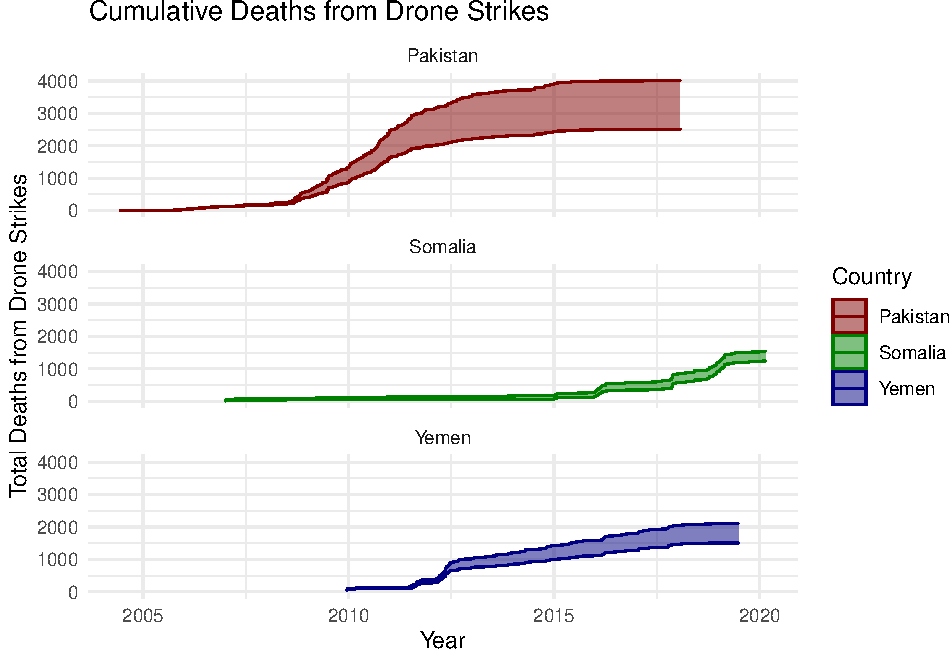
\includegraphics[width=0.75\linewidth]{strike-report_files/figure-latex/strike-deaths-1} \end{center}

\begin{center}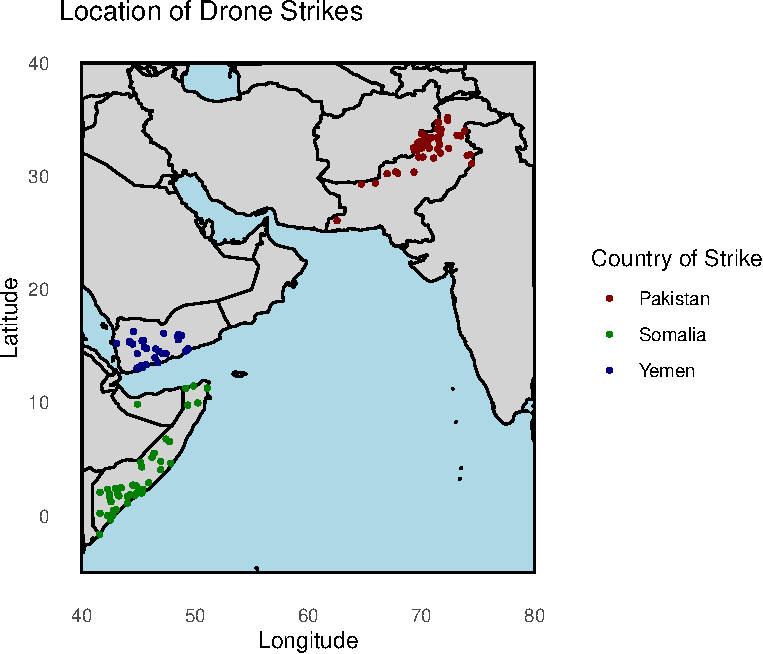
\includegraphics[width=0.75\linewidth]{strike-report_files/figure-latex/strike-location-1} \end{center}

\begin{center}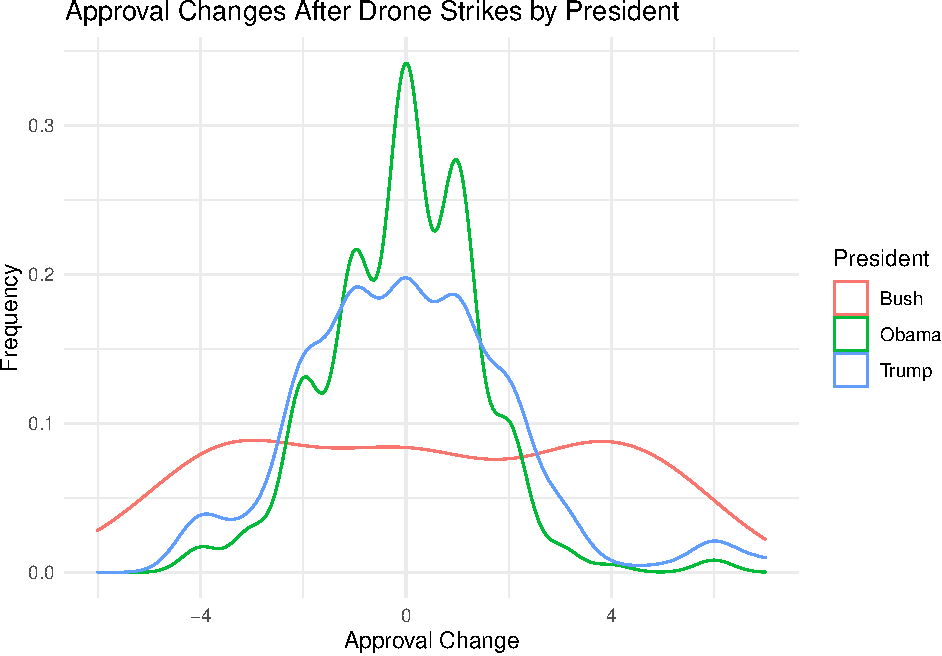
\includegraphics[width=0.75\linewidth]{strike-report_files/figure-latex/strike-approval-change-1} \end{center}

\hypertarget{statistical-analysis}{%
\section{Statistical Analysis}\label{statistical-analysis}}

After performing exploratory data analysis, we had three main interests
in the dataset: (1) the accuracy/effectiveness of the drone strikes (in
terms of casualties), (2) the strike lethality for each president, and
(3) the frequency of drone strikes for each president's term.

\hypertarget{drone-accuracy-rate}{%
\subsection{Drone Accuracy Rate}\label{drone-accuracy-rate}}

For this statistical analysis, we compared the three countries
(Pakistan, Somalia, and Yemen) with respect to the percentage of
civilian casualties. For the purposes of the analysis, we define the
total and civilian number of casualties as the average of the minimum
and maximum deaths for people and civilians, respectively.

We conducted the analysis as a Chi-squared test to look at the
distribution of civilian deaths across the three countries. Our null
hypothesis would assume that the distribution of civilian deaths matched
the distribution of noncivilian deaths, calculated by
\(\text{total deaths} - \text{civilian deaths}\). The reason we set the
null distribution as the number of noncivilians killed--and not just a
pure equality--is because the number of deaths does not remain
consistent across countries, so we wanted to account for that
distribution. We can summarize our null and alternative hypotheses as
follows:

\[
\begin{aligned}
H_0: & \text{ Civilian deaths follow the same distribution as noncivilian deaths}\\
H_a: & \text{ Civilian deaths do not follow the same distribution as noncivilian deaths}\\
\end{aligned}
\]

After conducting the Chi-squared test, we obtained a test statistic of
\(\chi^2 \approx 217.53\), which corresponds to a p-value of
\(p < 2.2 \times 10^{-16} \approx 0\). Thus, we reject our null
hypothesis that civilian deaths by country follow the same distribution
as noncivilian deaths, implying that the countries differed in the
accuracy of their strikes with respect to civilian deaths as a fraction
of total deaths. Moreover, a posthoc analysis of the test demonstrated
the stark differences on the country level:

\begin{table}[H]

\caption{\label{tab:drone_acc_posthoc}Posthoc Summary of Civilian Deaths by Country}
\centering
\begin{tabular}[t]{lrrrr}
\toprule
Country & Civilians Killed & Total Killed & Civilian Percent of Deaths & Pearson Residual\\
\midrule
Pakistan & 696 & 3,270 & 21.3\% & 9.3\\
Somalia & 72 & 1,390 & 5.2\% & -11.3\\
Yemen & 266 & 1,811 & 14.7\% & -1.6\\
\bottomrule
\end{tabular}
\end{table}

From the above posthoc analysis, we see that Pakistan had a decided
higher civilian death rate, while Somalia had a relatively low civilian
death rate. While we cannot make any causal inference from these
results, it appears that Pakistan--which does have data from an earlier
timeframe (since 2004)--has a less deliberate approach while Somalia had
greater accuracy in eliminating hostiles.

\hypertarget{drone-lethality}{%
\subsection{Drone Lethality}\label{drone-lethality}}

Our second analysis considered the lethality of drone strikes, by
president. Initially, when performing EDA, we noticed that the
distribution of deaths from drone strikes was heavily right-skewed. To
correct for this (and meet the assumptions for the ANOVA we wished to
conduct), we log-transformed the deaths after adding 1 to all deaths.
This ensured that we did not have to remove strikes with 0 deaths from
our analysis.

Once we ensured that we met the assumptions of our ANOVA, we could
construct our null and alternative hypotheses and conduct the analysis.
Our null hypothesis would be that the average number of deaths per
strike would be the same across all presidents; our alternative would be
that at least one president had a significantly different average number
of deaths.

\[
\begin{aligned}
H_0: & \text{ } \mu_\text{Bush} = \mu_\text{Obama} = \mu_\text{Trump} \\
H_a: & \text{ At least one } \mu \text{ is not equal} \\
\mu_\text{President} & \text{ represents the average number of deaths per strike, after transformation} \\
\end{aligned}
\]

\begin{table}[H]

\caption{\label{tab:drone_leth}ANOVA Results for Strike Lethality}
\centering
\begin{tabular}[t]{lrrrrr}
\toprule
  & df & SS & MS & F & p-value\\
\midrule
President & 2 & 53.89 & 26.94 & 44.93 & 0\\
Residuals & 941 & 564.31 & 0.60 &  & \\
\bottomrule
\end{tabular}
\end{table}

\begin{table}[H]

\caption{\label{tab:drone_leth_posthoc}TukeyHSD Pairwise Posthoc}
\centering
\begin{tabular}[t]{lr}
\toprule
Pairwise Comparison & Adjusted p-value\\
\midrule
Obama-Bush & 0.0245\\
Trump-Bush & 0.0000\\
Trump-Obama & 0.0000\\
\bottomrule
\end{tabular}
\end{table}
\begin{table}[H]

\caption{\label{tab:drone_leth_posthoc2}Lethality Statistics by President}
\centering
\begin{tabular}[t]{lrr}
\toprule
President & Average Deaths per Strike & Median Deaths per Strike\\
\midrule
Bush & 9.75 & 7.50\\
Obama & 7.03 & 5.00\\
Trump & 5.54 & 2.25\\
\bottomrule
\end{tabular}
\end{table}

\begin{center}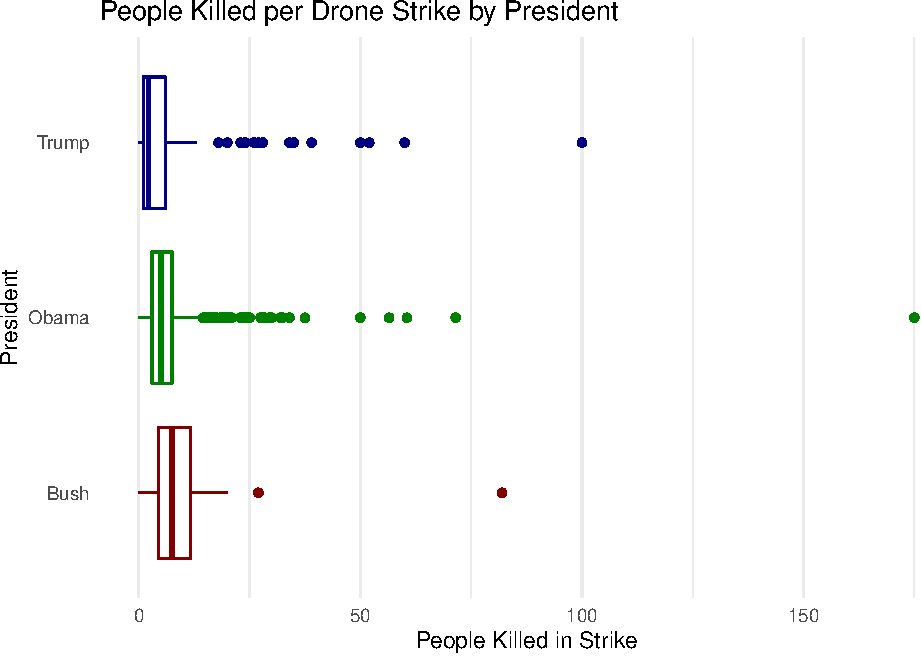
\includegraphics[width=0.75\linewidth]{strike-report_files/figure-latex/drone_leth_posthoc2-1} \end{center}

\hypertarget{drone-usage}{%
\subsection{Drone Usage}\label{drone-usage}}

Our third statistical analysis focused on the frequency of drone strike
usage by each president. However, this analysis had a much greater
limitation than our first analysis, due to the time frames for each
country. Thus, to accommodate for data discrepanies across countries, we
limited the date range to the overlapping date range across all three
datasets. After filtering the data, we had strikes from December 18,
2009 (\texttt{2009-12-18}) to January 18, 2018 (\texttt{2018-01-18}).
Because of this, our analysis for how frequently presidents utilized
drone only applies to Presidents Obama and Bush.

From here, we conducted another Chi-squared test to see if the frequency
of strikes aligned with the term length for each president over the
restricted time frame. Therefore, we can summarize our null and
alternative hypothesis as:

\[
\begin{aligned}
H_0: & \text{ The number of drone strikes follow the distribution of term length} \\
H_a: & \text{ The number of drone strikes do not follow the distribution of term length} \\
\end{aligned}
\]

After running the analysis, we obtained a Chi-squared statistic of
0.1316, which has a p-value of 0.7168. Thus, at the \(\alpha = 0.05\)
significance level, we fail to reject the null hypothesis--we do not
have sufficient evidence that the frequency of drone strikes differed
between Presidents Obama and Trump. However, as we noted earlier, this
analysis was severely constrained due to the shorter time frame that
overlapped across all three countries.

\hypertarget{dashboard}{%
\section{Dashboard}\label{dashboard}}

We expanded upon the basic graphics made in our exploratory data
analysis and added more complex visualizations for the RShiny dashboard.

Specifically, we borrowed the visualizations for the cumulative deaths
over time overall and by country. From these base plots, we added
filters for each country--and each president--so that an end user could
select which countries and presidential terms to highlight.

We also created a tab with an interactive timeline to visualize the
strikes locations over time. This visualization shows strikes over time
at their impact point (found through geocoding), with the size and color
correlating to the number of deaths caused by that strike.

The interactive timeline map presented itself as the most intensive
element of the dashboard--and the project.

\hypertarget{conclusions}{%
\section{Conclusions}\label{conclusions}}

\hypertarget{suggestions-for-future-research}{%
\subsection{Suggestions for Future
Research}\label{suggestions-for-future-research}}

Additional research into these drone strikes include looking at the
relationship to terrorism attacks, including whether or not U.S.
citizens or affiliates were affected by the attack. One strong data
source would be the \href{https://start.umd.edu/gtd/}{Global Terrorism
Database (GTD)}; we chose not to use this dataset because we wanted to
make our analysis and dashboard public, which would have required
payment (the data is only free for private research).

Another sector to investigate would be the impact of drone
strikes--either count, death rates, or injuries--on presidential
approval rating. From my high-level exploration, there appeared to be
limited-to-no relationship between approval change and various drone
statistics, but a deeper dive into these two elements could glean
previously undiscovered insights.

\hypertarget{limitations}{%
\subsection{Limitations}\label{limitations}}

The original dataset contained data on drone strikes from Pakistan,
Somalia, and Yemen. For Pakistan, the data begins in 2004; for Somalia
and Yemen, we do not have drone strike data before 2007. Therefore, any
temporal analysis may not be wholly accurate if comparing across
presidential terms or countries. This became an issue when comparing the
frequency of drone strikes for each president; in my analysis, I limited
the date range of interest between December 17, 2009 and January 24,
2018 because this was the range of dates for which all three countries
had drone strikes. Therefore, I could only compare the strike frequency
between Presidents Obama and Trump.

Additionally, for geocoding the areas and countries to derive a latitude
and longitude, we used a Google Maps API. While useful, we remained
unable to geocode some locations due to undefined areas or incorrectly
mapped locations. To verify that the geocoded location was correct, we
redetermined the spatial country location from the latitude and
longitude. If the spatial country and the original country did not
match, we assigned the latitude and longitude to \texttt{NA} and dropped
those strikes from map visualizations. In total, we removed 109 of 944
drone strikes (11.55\%) for the map visualizations. However, we still
included these strikes in subsequent analyses.

In the analyses, we encountered a big limitation in the date range for
the individual countries. To avoid issues that may arise due to
missing/unaccounted data, we decided to bound the range of interest.
However, when doing this, we constricted Trump's term to approximately
one year and completely eliminated Bush, presenting a clear drawback of
that analysis.

\pagebreak

\hypertarget{sources}{%
\section{Sources}\label{sources}}

\hypertarget{data}{%
\subsection{Data}\label{data}}

\begin{itemize}
\tightlist
\item
  The Guardian (via Professor Vivian Lew, UCLA Department of Statistics)

  \begin{itemize}
  \tightlist
  \item
    \texttt{us-pakistan-strikes-from-2004.xlsx}
  \item
    \texttt{us-somalia-strikes-from-2007.xlsx}
  \item
    \texttt{us-yemen-strikes-from-2007.xlsx}
  \end{itemize}
\item
  Gallup (via
  \href{https://www.presidency.ucsb.edu/statistics/data/presidential-job-approval-all-data}{UCSB})

  \begin{itemize}
  \tightlist
  \item
    \texttt{bush-ratings.csv}
  \item
    \texttt{obama-ratings.csv}
  \item
    \texttt{trump-ratings.csv}
  \end{itemize}
\end{itemize}

\hypertarget{help-websites}{%
\subsection{Help Websites}\label{help-websites}}

\begin{itemize}
\tightlist
\item
  \href{https://stackoverflow.com/questions/14334970/convert-latitude-and-longitude-coordinates-to-country-name-in-r}{Creating
  spatial mapping in R from coordinates}
\item
  \href{https://towardsdatascience.com/eye-catching-animated-maps-in-r-a-simple-introduction-3559d8c33be1}{Creating
  an RShiny map timeline}
\end{itemize}

\hypertarget{r-packages}{%
\subsection{R Packages}\label{r-packages}}

\begin{itemize}
\tightlist
\item
  \texttt{ggmap}: D. Kahle and H. Wickham. ggmap: Spatial Visualization
  with ggplot2. The R Journal, 5(1), 144-161. URL
  \url{http://journal.r-project.org/archive/2013-1/kahle-wickham.pdf}
\item
  \texttt{lubridate}: Garrett Grolemund, Hadley Wickham (2011). Dates
  and Times Made Easy with lubridate. Journal of Statistical Software,
  40(3), 1-25. URL \url{https://www.jstatsoft.org/v40/i03/}.
\item
  \texttt{readxl}: Hadley Wickham and Jennifer Bryan (2022). readxl:
  Read Excel Files. R package version 1.4.0.
  \url{https://CRAN.R-project.org/package=readxl}
\item
  \texttt{rvest}: Hadley Wickham (2021). rvest: Easily Harvest (Scrape)
  Web Pages. R package version 1.0.2.
  \url{https://CRAN.R-project.org/package=rvest}
\item
  \texttt{rworldxtra}: Andy South (2012). rworldxtra: Country boundaries
  at high resolution.. R package version 1.01.
  \url{https://CRAN.R-project.org/package=rworldxtra}
\item
  \texttt{sp}: Pebesma, E.J., R.S. Bivand, 2005. Classes and methods for
  spatial data in R. R News 5 (2),
  \url{https://cran.r-project.org/doc/Rnews/}.
\item
  \texttt{tidyverse}: Wickham et al., (2019). Welcome to the tidyverse.
  Journal of Open Source Software, 4(43), 1686,
  \url{https://doi.org/10.21105/joss.01686}
\end{itemize}

\end{document}
